\section{Methods}
\subsection{Problem Setup and Offline--Online Framework}
Let $\mathcal D=\{(x_i,t_i,y_i)\}_{i=1}^N$ denote a training set of radiographs $x_i$, clinical histories $t_i$, and labels $y_i\in\{1,\ldots,K\}$. XBone-Net initializes its image and text encoders from BiomedCLIP~\cite{BiomedCLIP}. We denote their global tokens by $v_0,t_0$ and remaining token sequences by $V_\ell,T_\ell$.

The framework has two offline phases. Phase~1 adapts the encoders through class-aware image--text alignment. Phase~2 learns bidirectional token fusion and supervised classification from the adapted encoders. Validation data select the checkpoint in each phase. Online inference applies the saved preprocessing and fixed Phase-2 weights to an image--history pair, returning class probabilities and the predicted label.

LoRA~\cite{Hu2022LoRA} restricts encoder updates to adapters in attention and feed-forward projections. For a frozen pretrained matrix $W_0$, the adapted weight is
\begin{equation}
W=W_0+\frac{\alpha}{r}BA,\quad
A\in\mathbb R^{r\times d_i},\quad B\in\mathbb R^{d_o\times r}.
\label{eq:lora}
\end{equation}
We use rank $r=16$, scaling $\alpha=32$, and adapter dropout 0.1.

\subsection{Phase 1: Class-Aware Image--Text Alignment}
Phase~1 learns image--text correspondence before fusion and classification (Fig.~\ref{fig:phase1}). Each full batch contains two examples from each of eight sampled classes. Beyond the observed pairs, the objective assigns partial positive weight to unpaired examples of the same diagnostic class. For a batch of $B$ pairs, the soft matching weights are
\begin{equation}
A_{ij}=\ind[i=j]+\rho\ind[i\ne j,\ y_i=y_j],\quad \rho=0.5.
\end{equation}
The observed pair receives weight one, another pair of the same class receives weight $\rho$, and different-class pairs receive zero. Row and column normalization yield
\begin{equation}
Q^{I\to T}_{ij}=\frac{A_{ij}}{\sum_{k=1}^B A_{ik}},\qquad
Q^{T\to I}_{ji}=\frac{A_{ij}}{\sum_{k=1}^B A_{kj}}.
\end{equation}
For $L_2$-normalized global embeddings $\bar v_i,\bar t_j$, the similarity logit is
\begin{equation}
C_{ij}=e^s\bar v_i^\top\bar t_j,
\end{equation}
where $s$ is the fixed pretrained logit scale. Row-wise softmax of $C$ and $C^\top$ gives $P^{I\to T}$ and $P^{T\to I}$. Inspired by semantic matching~\cite{MedCLIP}, we minimize
\begin{equation}
\mathcal L_{\mathrm{SM}}=-\frac{1}{2B}\sum_{i=1}^B\sum_{j=1}^B
\left[Q^{I\to T}_{ij}\log P^{I\to T}_{ij}
+Q^{T\to I}_{ji}\log P^{T\to I}_{ji}\right].
\label{eq:align}
\end{equation}
This objective encourages class-consistent correspondence while retaining the observed pair as the strongest match. Class identity supplies a coarse similarity prior and does not imply that two cases have identical anatomy, severity, or history.

\begin{figure}[t]
\centering
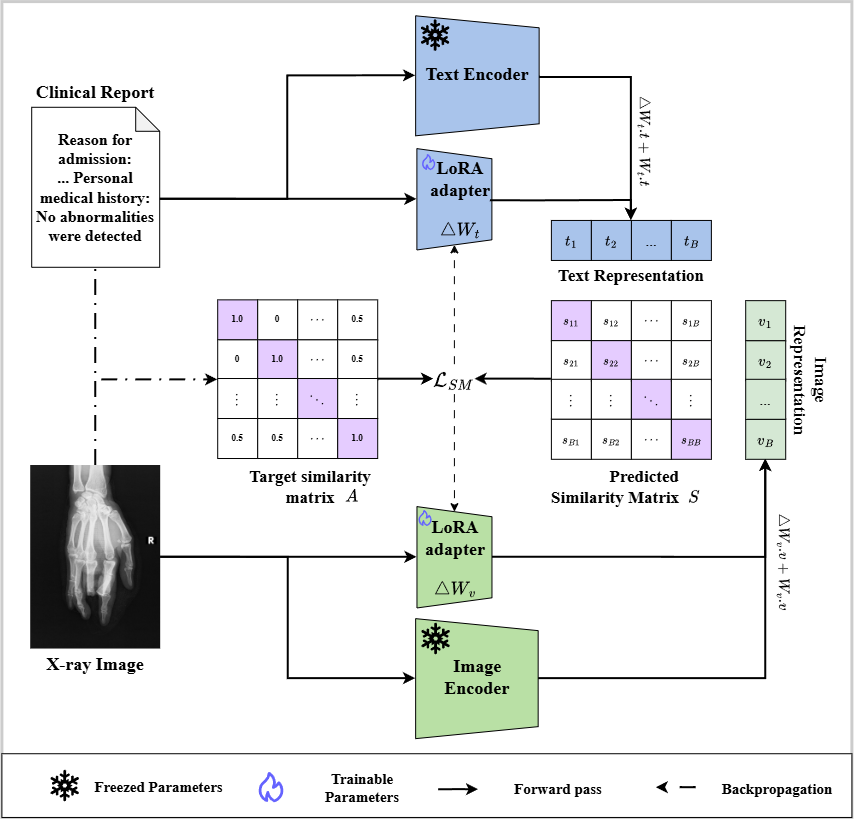
\includegraphics[width=\columnwidth]{phase1.png}
\caption{Phase 1: class-aware image--text alignment with soft matching targets. The pretrained encoder weights remain frozen while the LoRA adapters are optimized.}
\label{fig:phase1}
\end{figure}

\subsection{Phase 2: Bidirectional Fusion and Classification}
Phase~2 uses the encoders' native token sequences (Fig.~\ref{fig:phase2}). Tokens are layer-normalized and projected to 512 dimensions, with additional normalization of global tokens. Each global token queries the other modality's local tokens through eight-head attention. Reusing the token notation for these transformed features, the residual summaries are
\begin{equation}
\begin{aligned}
h_I&=\operatorname{LN}\big(v_0+\operatorname{Drop}(\operatorname{MHA}(v_0,T_\ell,T_\ell;M_T))\big),\\
h_T&=\operatorname{LN}\big(t_0+\operatorname{Drop}(\operatorname{MHA}(t_0,V_\ell,V_\ell))\big),
\end{aligned}
\label{eq:fusion}
\end{equation}
where $M_T$ masks text padding. Thus, image features condition the selection of textual features and history conditions the selection of visual features. The summaries pass through a $1024\to512\to512$ MLP with GELU and dropout, followed by a linear classifier:
\begin{equation}
z=\operatorname{LN}(\operatorname{MLP}([h_I;h_T])),\quad
p=\operatorname{softmax}(W_cz+b_c).
\end{equation}

The supervised objective combines effective-number class weighting~\cite{Cui2019ClassBalanced} with label smoothing. For class $c$ with $n_c$ training examples, define its effective number and inverse weight as
\begin{equation}
E_c=\frac{1-\beta^{n_c}}{1-\beta},\qquad a_c=E_c^{-1},\quad\beta=0.999.
\end{equation}
The normalized weight is clipped at five:
\begin{equation}
w_c=\min\left(\frac{Ka_c}{\sum_j a_j},5\right).
\end{equation}
Label smoothing regularizes the target distribution:
\begin{equation}
u_{ic}=(1-\epsilon)\ind[y_i=c]+\frac{\epsilon}{K},\qquad\epsilon=0.1.
\end{equation}
The resulting weighted cross-entropy is
\begin{equation}
\mathcal L_{\mathrm{cls}}=-\frac{\sum_i\sum_c w_cu_{ic}\log p_{ic}}{\sum_i w_{y_i}},
\label{eq:loss}
\end{equation}
where $p_{ic}$ is the predicted class probability. Weights use training counts only and apply to all smoothed target terms. Phase~2 updates adapters, fusion, and the classifier while pretrained encoder weights remain frozen. Individual effects of weighting and smoothing require separate ablations.

\begin{figure}[t]
\centering
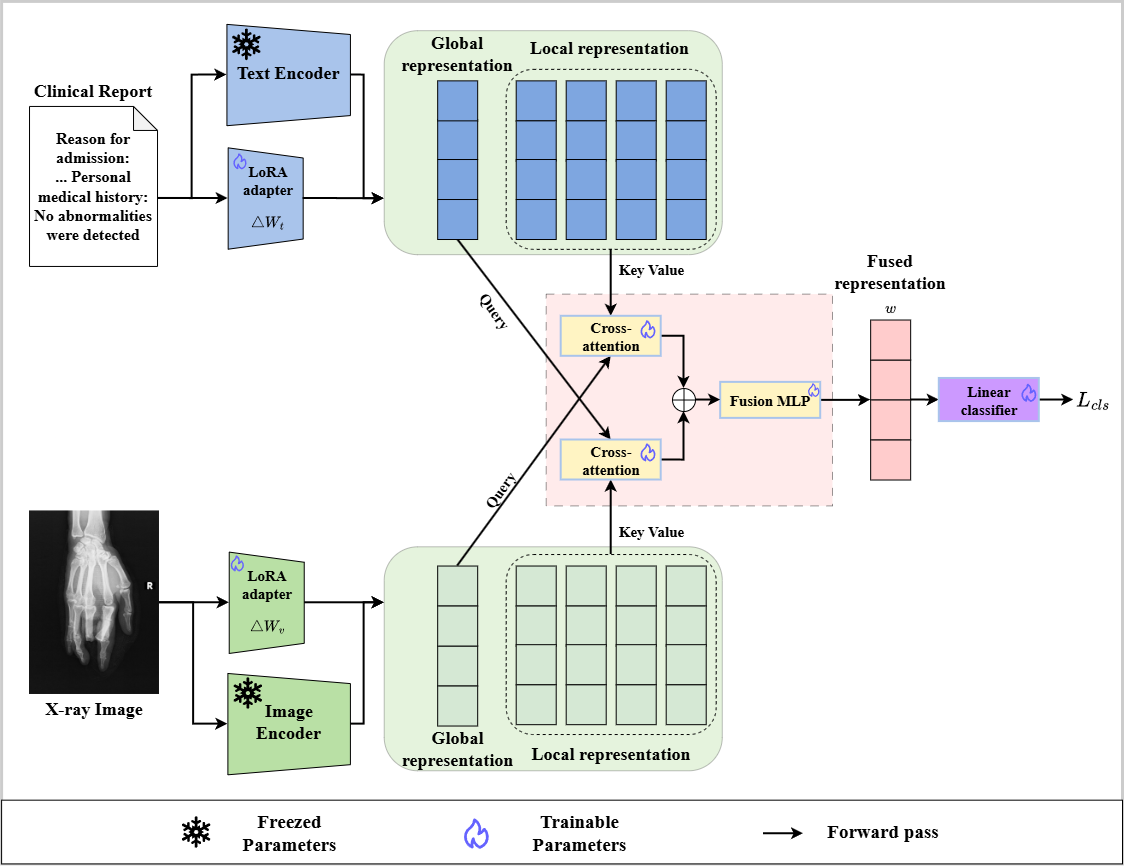
\includegraphics[width=\columnwidth]{phase2.png}
\caption{Phase 2: bidirectional global-to-local fusion and classification, initialized with the Phase-1 adapters. The selected model supplies fixed-weight online inference.}
\label{fig:phase2}
\end{figure}

\subsection{Integrated Gradients Attribution}
Integrated Gradients (IG)~\cite{Sundararajan2017IntegratedGradients} attributes the original predicted-class logit $F_{\hat y}$ to input components relative to reference $u^0$:
\begin{equation}
\operatorname{IG}_j(u,u^0)=(u_j-u_j^0)\int_0^1
\frac{\partial F_{\hat y}(u^0+\lambda(u-u^0))}{\partial u_j}\,d\lambda.
\end{equation}
We hold the other modality fixed. The image reference is the zero tensor in normalized image space, whereas the text reference replaces content embeddings with padding embeddings while preserving special tokens and masks. Attribution-ranked deletion measures changes in the original predicted-class probability. Deletion AUC integrates this probability over the fraction removed. These interventions characterize input dependence under the specified references without establishing lesion localization or clinical correctness.
